\documentclass[11pt,a4paper,twoside]{article}
\usepackage{lmodern}
\usepackage{amssymb,amsmath}
\usepackage{ifxetex,ifluatex}
\usepackage{fixltx2e} % provides \textsubscript
\ifnum 0\ifxetex 1\fi\ifluatex 1\fi=0 % if pdftex
  \usepackage[T1]{fontenc}
  \usepackage[utf8]{inputenc}
\else % if luatex or xelatex
  \ifxetex
    \usepackage{mathspec}
  \else
    \usepackage{fontspec}
  \fi
  \defaultfontfeatures{Ligatures=TeX,Scale=MatchLowercase}
\fi
% use upquote if available, for straight quotes in verbatim environments
\IfFileExists{upquote.sty}{\usepackage{upquote}}{}
% use microtype if available
\IfFileExists{microtype.sty}{%
\usepackage{microtype}
\UseMicrotypeSet[protrusion]{basicmath} % disable protrusion for tt fonts
}{}
\usepackage[left=2.5cm,right=3.5cm,top=83.75pt,textheight=24.35cm,textwidth=15cm,a4paper,headheight=13.6pt,twoside=true]{geometry}
\usepackage{hyperref}
\hypersetup{unicode=true,
            pdfborder={0 0 0},
            breaklinks=true}
\urlstyle{same}  % don't use monospace font for urls
\usepackage{biblatex}

\addbibresource{bibliography.bib}
\addbibresource{packages.bib}
\usepackage{longtable,booktabs}
\usepackage{graphicx,grffile}
\makeatletter
\def\maxwidth{\ifdim\Gin@nat@width>\linewidth\linewidth\else\Gin@nat@width\fi}
\def\maxheight{\ifdim\Gin@nat@height>\textheight\textheight\else\Gin@nat@height\fi}
\makeatother
% Scale images if necessary, so that they will not overflow the page
% margins by default, and it is still possible to overwrite the defaults
% using explicit options in \includegraphics[width, height, ...]{}
\setkeys{Gin}{width=\maxwidth,height=\maxheight,keepaspectratio}
\IfFileExists{parskip.sty}{%
\usepackage{parskip}
}{% else
\setlength{\parindent}{0pt}
\setlength{\parskip}{6pt plus 2pt minus 1pt}
}
\setlength{\emergencystretch}{3em}  % prevent overfull lines
\providecommand{\tightlist}{%
  \setlength{\itemsep}{0pt}\setlength{\parskip}{0pt}}
\setcounter{secnumdepth}{5}

%%% Use protect on footnotes to avoid problems with footnotes in titles
\let\rmarkdownfootnote\footnote%
\def\footnote{\protect\rmarkdownfootnote}

%%% Change title format to be more compact
\usepackage{titling}

% Create subtitle command for use in maketitle
\newcommand{\subtitle}[1]{
  \posttitle{
    \begin{center}\large#1\end{center}
    }
}

\setlength{\droptitle}{-2em}

  \title{}
    \pretitle{\vspace{\droptitle}}
  \posttitle{}
    \author{}
    \preauthor{}\postauthor{}
    \date{}
    \predate{}\postdate{}
  
\usepackage{booktabs}
\usepackage[ngerman,english]{babel} % deutsche Trennregeln, "Inhaltsverzeichnis" etc.
\usepackage{mathptmx} % Times-Roman-Schrift (auch für mathematische Formeln)
% \usepackage{pdfpages}
% \usepackage{pgf}
% \usepackage{epstopdf}

\usepackage[labelfont=bf]{caption}
% \usepackage{changepage}
% \usepackage{subcaption}
% \usepackage{hanging}

\usepackage{array}

\usepackage{epigraph}
\renewcommand{\epigraphsize}{\small}
\setlength{\epigraphwidth}{.6\textwidth}

% custom imports
% multirows für Tabellen
% \usepackage{multirow}
% nice quotes
\usepackage[autostyle=true,german=quotes]{csquotes}

\usepackage[onehalfspacing]{setspace} % 1,5facher Zeilenabstand

% Zum Setzen von URLs
\usepackage{color}
\definecolor{darkred}{rgb}{0.25,0,0}
\definecolor{darkgreen}{rgb}{0,0.2,0}
\definecolor{darkmagenta}{rgb}{0.2,0,0.2}
\definecolor{darkcyan}{rgb}{0,0.15,0.15}

\usepackage{fancyhdr} % Positionierung der Seitenzahlen

\renewcommand{\headrulewidth}{0pt}

% Korrektes Format für Nummerierung von Abbildungen (figure) und
% Tabellen (table): <Kapitelnummer>.<Abbildungsnummer>
\makeatletter
\@addtoreset{figure}{section}
\renewcommand{\thefigure}{\thesection.\arabic{figure}}
\@addtoreset{table}{section}
\renewcommand{\thetable}{\thesection.\arabic{table}}
\makeatother

% include bibliography in ToC - special case for biblatex (bookdown doesn't handle this atm)
\let\oldpb\printbibliography
\renewcommand{\printbibliography}{\oldpb[heading=bibintoc]}

\let\oldpar\paragraph
\renewcommand{\paragraph}{\oldpar*}

\let\oldsubpar\subparagraph
\renewcommand{\subparagraph}{\oldsubpar*}

%\sloppy % Damit LaTeX nicht so viel über "overfull hbox" u.Ä. meckert

% römische numerale für Inhaltsverzeichnis; wird in index.Rmd zurückgesetzt
\fancyhead[LE,RO,LO,RE]{}
\fancyfoot[CE,CO,RE,LO]{}
\fancyfoot[LE,RO]{\roman{page}}

\begin{document}

\pagestyle{empty} % Vorerst keine Seitenzahlen
\pagenumbering{alph} % Unsichtbare alphabetische Nummerierung

\begin{center}
\textsc{Ludwig-Maximilians-Universität München}\\
Department ``Institut für Informatik''\\
Professur für Computational Social Science and Big Data\\
Prof.\ Jürgen Pfeffer

\vspace{4.75cm}
{\large\textbf{Masterarbeit}}\vspace{.5cm}

{\Huge{}Not all those who wander are lost}\\\vspace{.5cm}
{\Large{}Dynamiken bei der Interessensentwicklung in Online Communities}\vspace{.75cm}

{\large Oliver Baumann}\\\href{mailto:baumanno@cip.ifi.lmu.de}{<baumanno@cip.ifi.lmu.de>}

\end{center}
\vfill

\begin{tabular}{ll}
Bearbeitungszeitraum: & 30.04.2018 bis 29.10.2018\\
Betreuer: & Dr.\ Mirco Schönfeld\\
Verantw. Hochschullehrer: & Prof.\ Jürgen Pfeffer
\end{tabular}

%______________________________________________________________________

\clearpage
\section*{Zusammenfassung}

Die vorliegende Arbeit reiht sich in Forschungsliteratur zu interaktiven Tischen, interaktiven Arbeitsumgebungen,
gekrümmten Multitouch-Displays und indirekten Multitouch-Mappings ein. Anhand einer Nutzerstudie wird die Wirkung zweier indirekter
Eingabemodi auf den Nutzer untersucht. Dazu wurde für \emph{Curve}, ein interaktiver Tisch mit gebogenem Display,
eine prototypische Anwendung entwickelt, die entweder mit einer Maus oder über Multitouch-Gesten bedient werden kann.
Im Gegensatz zu isolierten Tasks ermöglicht die Anwendung den von einer Desktopumgebung gewohnten Arbeitsablauf. Das System
bietet für den Anwendungsfall "`Audio-Bearbeitung"' die Möglichkeit, in einem Audio-Sample zu navigieren und dieses
zu modifizieren. Die beiden Interface-Varianten wurden auf ihre Wirkung auf das Nutzererlebnis und ihre Eignung
zum Einsatz in interaktiven Arbeitsplätzen hin untersucht. Es wurde festgestellt, dass keine der beiden Varianten
dabei übermäßig gut oder schlecht abschneidet. Beide Eingabetechniken sind dabei ähnlich gut für den speziellen
Anwendungsfall geeignet. Ein Transfer zu anderen Einsatzmöglichkeiten schließt die Arbeit ab. Es sei darauf hingewiesen,
dass die in dieser Studie präsentierten Ergebnisse anhand einer kleinen Stichprobe ermittelt wurden und möglicherweise
nicht vollends generalisierbar sind.

\iffalse
\selectlanguage{english}
\section*{Abstract}

We relate in parts to previous work on interactive desks, interactive workspaces, bent multitouch-enabled displays
and indirect mappings for multitouch. Based on a user-study, we compare the effects of two interaction techniques on the user.
To this end, we implemented a prototypical application for \emph{Curve}, an interactive desk with a bent multitouch-display.
The user can interact with the application either via a mouse, or via multitouch-gestures.
In contrast to isolated tasks commonly used, our system enables a workflow comparable to that of a traditional desktop
environment. The system relates to the specific use-case of audio-editing and allows for navigating and manipulating an audio-sample.
Both interaction techniques presented here have been studied with regard to their effect on user experience and their
compatibility with being used in interactive workspaces. We conclude that neither of the two techniques out- or underperforms
and thus suggest that they are equally suitable for this particular use case. We end with suggesting other possible applications
of this setup, not restricted to any single use-case. We note, however, that due to the small sample size of our study, the
findings presented here might not be fully generalizable.
\selectlanguage{ngerman}
\fi
\clearpage
\section*{Eidesstattliche Erklärung}

\selectlanguage{ngerman}

\noindent Ich erkläre hiermit, dass ich die vorliegende Arbeit
selbstständig angefertigt, alle Zitate als solche kenntlich gemacht
sowie alle benutzten Quellen und Hilfsmittel angegeben habe.

\vspace{7ex}
\noindent\makebox[9.3cm]{\dotfill}

\smallskip\noindent München, \today

%______________________________________________________________________

\cleardoublepage

\pagestyle{fancy}
\pagenumbering{roman} % Römische Seitenzahlen
\setcounter{page}{1}

{
\setcounter{tocdepth}{3}
\tableofcontents
}
\cleardoublepage

\pagenumbering{arabic}
\setcounter{page}{1}

\fancyhead[LE,RO]{\rightmark}
\fancyhead[LO,RE]{\leftmark}
\fancyfoot[LE,RO]{\thepage}

\cleardoublepage

\hypertarget{einleitung}{%
\section{Einleitung}\label{einleitung}}

\epigraphhead[80]{\epigraph{The world is a thing of utter inordinate complexity and richness and strangeness that is absolutely awesome.}{\textit{Douglas Adams}}}

\cleardoublepage

\hypertarget{grundlagen-und-verwandte-forschung}{%
\section{Grundlagen und verwandte
Forschung}\label{grundlagen-und-verwandte-forschung}}

\hypertarget{topic-modelle}{%
\subsection{Topic-Modelle}\label{topic-modelle}}

\hypertarget{lda}{%
\subsubsection{LDA}\label{lda}}

\hypertarget{verwandte-arbeiten}{%
\subsubsection{Verwandte Arbeiten}\label{verwandte-arbeiten}}

\hypertarget{soziale-netzwerkanalyse}{%
\subsection{Soziale Netzwerkanalyse}\label{soziale-netzwerkanalyse}}

\hypertarget{graphen-und-netzwerke}{%
\subsubsection{Graphen und Netzwerke}\label{graphen-und-netzwerke}}

\hypertarget{ego-netzwerke}{%
\subsubsection{Ego-Netzwerke}\label{ego-netzwerke}}

\hypertarget{verwandte-arbeiten-1}{%
\subsubsection{Verwandte Arbeiten}\label{verwandte-arbeiten-1}}

\hypertarget{reddit}{%
\subsection{Reddit}\label{reddit}}

\hypertarget{begriffsklarung}{%
\subsubsection{Begriffsklärung}\label{begriffsklarung}}

\hypertarget{verwandte-arbeiten-2}{%
\subsubsection{Verwandte Arbeiten}\label{verwandte-arbeiten-2}}

\cleardoublepage

\hypertarget{datenanalyse}{%
\section{Datenanalyse}\label{datenanalyse}}

Dieses Kapitel liefert einen Überblick über die Methodik sowie die
Ergebnisse der Datenanalyse. Zunächst wird der verwendete Datensatz
präsentiert und Kritik daran erörtert. Weiterhin wird dargelegt, wie die
betrachteten Topic-Modelle erzeugt werden und welche Methoden der
sozialen Netzwerkanalyse Anwendung finden, sowie welche
Software-Komponenten jeweils zum Einsatz kommen. Im zweiten Teil des
Kapitels werden dann die Ergebnisse vorgestellt, ohne dabei jedoch einer
Interpretation zu weit vorzugreifen.

\hypertarget{methodik}{%
\subsection{Methodik}\label{methodik}}

\hypertarget{datensatz}{%
\subsubsection{Datensatz}\label{datensatz}}

Die Grundlage der Analyse bildet ein frei zugänglicher Datensatz mit
Reddit-Kommentaren. Jason Baumgartner, der unter dem Pseudonym
\emph{stuck\_in\_the\_matrix}\footnote{\url{https://www.reddit.com/user/stuck_in_the_matrix}}
selbst auf Reddit aktiv ist, stellt monatliche Zusammenfassungen aller
erstellten Kommentare zum Download bereit \autocite{Baumgartner}. Diese
reichen zum gegenwärtigen Zeitpunkt von Oktober 2018 zurück bis Dezember
2005.

\hypertarget{struktur}{%
\paragraph{Struktur}\label{struktur}}

Die monatlichen Datensätze liegen in Form von Textdateien vor, in denen
jede Zeile einen Kommentar sowie Metadaten enthält. Das maschinenlesbare
JSON-Format, in dem die Daten abgelegt sind, ermöglicht dabei eine
effiziente computergestützte Auswertung. Tabelle \ref{tab:importantkeys}
führt die für diese Arbeit relevanten Schlüssel-Wert-Paare des
Datensatzes auf. Der Schlüssel \emph{parent\_id} bezeichnet dabei das
Element, auf welches sich der Kommentar bezieht. Dies können Beiträge
oberster Ordnung sein, sog. \enquote{Links}, oder selbst Kommentare
\autocite{Reddit2018}. Zu beachten ist hier insbesondere, dass der
eigentliche Textinhalt des Kommentars für diese Auswertung nicht genutzt
wird.

\begin{table}

\caption{\label{tab:importantkeys}wichtige Schlüssel-Wert-Paare des Datensatzes}
\centering
\begin{tabular}[t]{ll}
\toprule
Schlüssel & Wert\\
\midrule
author & Nutzername des Kommentar-Erstellers\\
id & eindeutige ID des Kommentars\\
parent\_id & eindeutige ID des Elements, auf das sich der Kommentar bezieht\\
subreddit & Name des Subreddits, in dem der Kommentar erstellt wurde\\
\bottomrule
\end{tabular}
\end{table}

\hypertarget{koharenz-des-datensatzes}{%
\paragraph{Kohärenz des Datensatzes}\label{koharenz-des-datensatzes}}

Im März 2018 haben Gaffney und Matias eine Analyse des
Baumgartner-Korpus vorgelegt \autocite{Gaffney2018}. Der vollständige
Korpus enthält neben Kommentaren auch Datensätze mit allen monatlich
erstellten Beiträgen, im folgenden auch \enquote{Submissions} genannt.
Gaffney und Matias kommen zu dem Schluss, dass die Erfassung sowohl der
Submissions als auch der Kommentare Lücken aufweist, also Elemente
gänzlich nicht im Datensatz vorhanden sind. Für den Gegenstand der
vorliegenden Arbeit ist dieser Umstand insofern von Bedeutung, als dass
fehlende Kommentare die Topic-Affinität von Nutzern verzerren können,
etwa wenn ein Topic, in dem der Nutzer durchaus aktiv war, aufgrund
fehlender Daten unterrepräsentiert ist. Auch Gaffney und Matias stellen
fest, dass Studien, welche auf die vollständige Historie von Nutzern
zugreifen, dem höchsten Risiko ausgesetzt sind, lückenhafte Daten zu
betrachten \autocite{Gaffney2018}.

Reddit weist jedem Kommentar eine eindeutige numerische ID zu. Das von
Baumgartner eingesetzte System nimmt zusammenhängende Blöcke von jeweils
100 solcher IDs und versucht, die zugehörigen Kommentare über die
Reddit-API\footnote{\url{https://api.reddit.com/}} aufzulösen
\autocite{Baumgartner2018a}. Da Reddit auch Anfragen nach gelöschten
Elementen sinnvoll beantwortet, also nicht etwa mit einer Fehlermeldung,
sollte ein Bereich von 100 sequentiellen IDs auch vollständig im
Datensatz abgebildet sein, inklusive als gelöscht markierter Elemente.
Gaffney und Matias stellen jedoch für den Zeitraum Dezember 2005 bis
Februar 2016 fest, dass 943.755 Kommentar- und 1.539.583 Beitrags-IDs
nicht in den Datensätzen enthalten sind. Als mögliche Gründe für das
Fehlen nennen Gaffney und Matias dreierlei: sog. \enquote{dangling
references}, also Verweise, bei denen das Element, auf das verwiesen
wird, nicht auffindbar ist; öffentlich zugängliche Daten, die aus
unbekanntem Grund nicht von Reddit an Baumgartners System übertragen
wurden; oder Daten aus als privat eingestuften Communities, die nicht
öffentlich sondern nur von Mitgliedern mit Zugangsberechtigung einsehbar
sind \autocite{Gaffney2018}.







\begin{figure}

{\centering 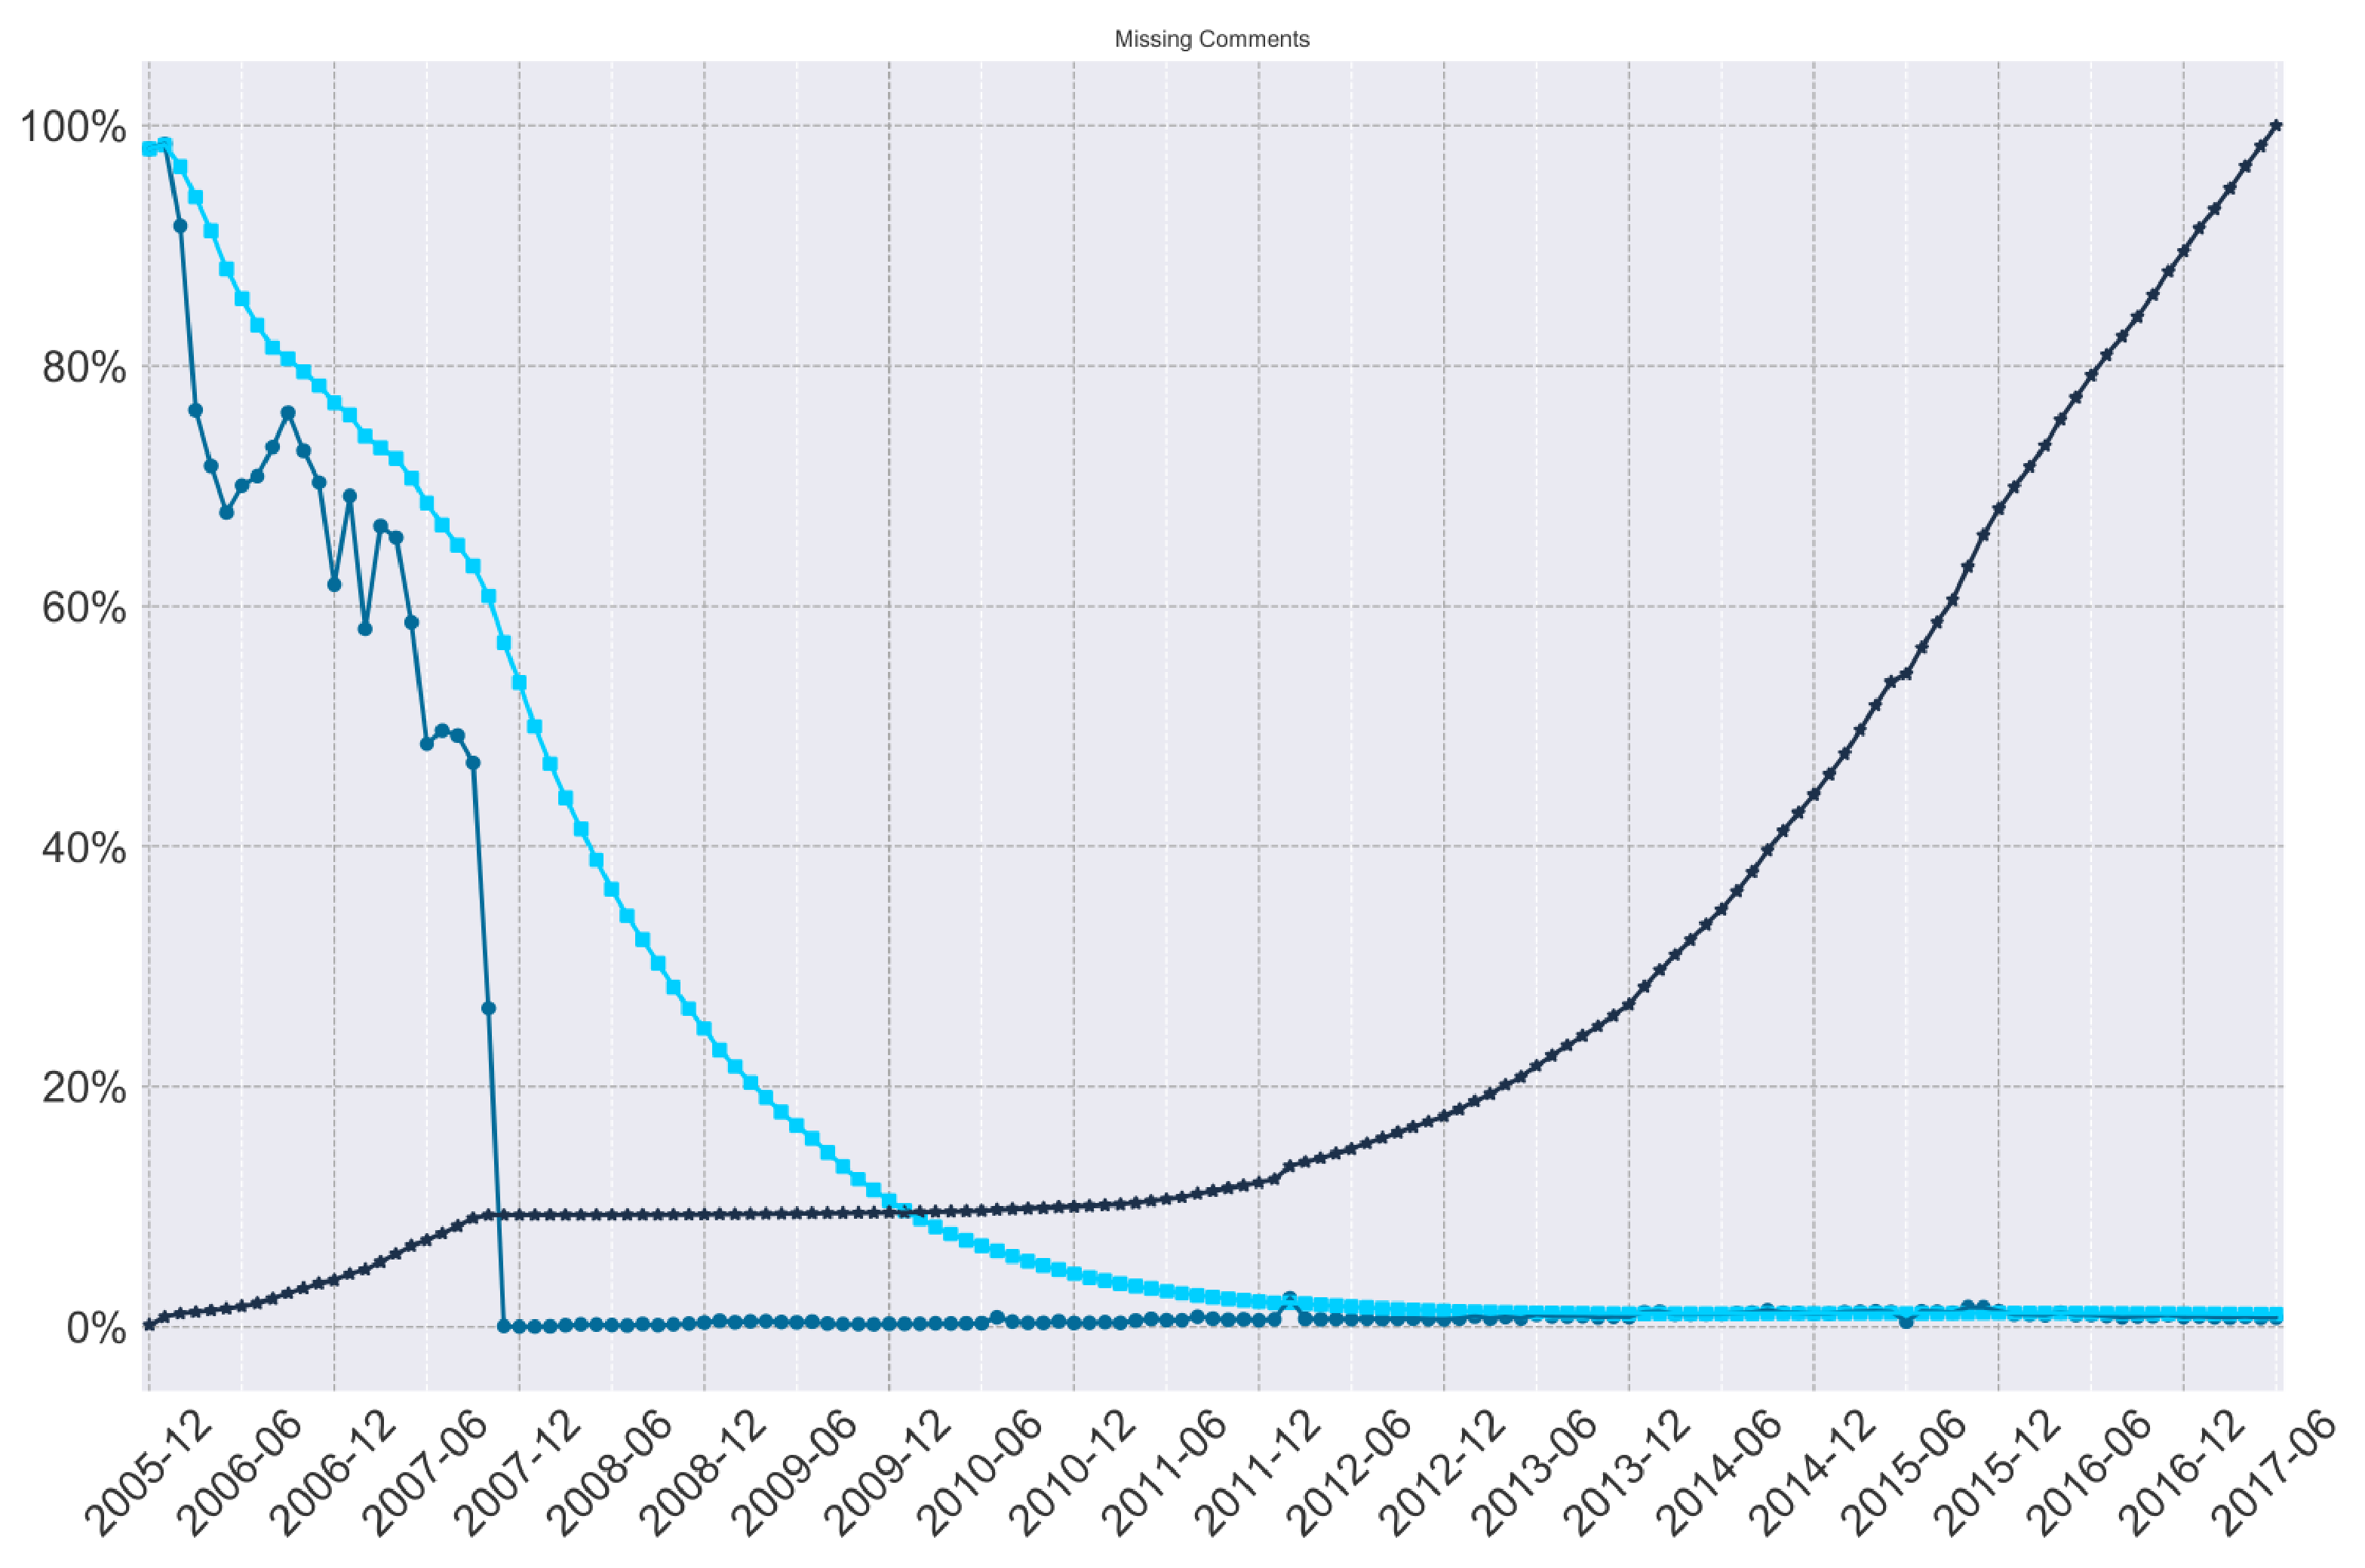
\includegraphics[width=0.75\linewidth]{./images/gaffneymatias_fig4} 

}

\caption{Anteil fehlender Kommentare. Die hellblauen Quadrate (obere
Linie) stellen den gleitenden Mittelwert fehlender Kommentare in Prozent
dar, die mittelblauen Punkte (mittlere Linie) den prozentualen Anteil
fehlender Kommentare, und die dunkelblauen Kreuze (untere Linie) die
kumulierte Gesamtzahl fehlender Kommentare \autocite{Gaffney2018}}\label{fig:gf4}
\end{figure}

In Abbildung \ref{fig:gf4} stellen die mittelblauen Punkte den Anteil
fehlender Kommentare in Prozent dar. Ab etwa April 2006 beginnt dieser
Anteil zu sinken, fällt ab etwa August 2007 stark ab und stabilisiert
sich ab etwa November 2007 im niedrigen einstelligen Bereich. Um den
Einfluss fehlender Kommentare so gering wie möglich zu halten, wurden
daher für die vorliegende Arbeit die Datensätze beginnend mit November
2007 bis einschließlich Februar 2018 ausgewertet.\\
Jason Baumgartner hat als Folge der Veröffentlichung von Gaffney und
Matias angekündigt, fehlende Kommentare und Beiträge nachträglich zu
erfassen \autocite{Baumgartner2018}.

\hypertarget{stichprobe-von-nutzern}{%
\subsubsection{Stichprobe von Nutzern}\label{stichprobe-von-nutzern}}

Nachdem der Datensatz einer zeitlichen Einschränkung unterworfen wurde,
müssen Kriterien für die Auswahl von Nutzern herangezogen werden. Dieser
Abschnitt gibt Aufschluss über die Altersverteilung von Nutzern im
Datensatz und beschreibt die Ziehung einer Stichprobe für die
Datenanalyse.

\hypertarget{altersverteilung}{%
\paragraph{Altersverteilung}\label{altersverteilung}}

Nach der zeitlichen Eingrenzung der Daten liegen für den betrachteten
Zeitraum von 124 Monaten etwa 3,6 Milliarden Kommentare vor, verfasst
von ca. 28 Millionen Nutzern. Für jeden dieser Nutzer wurde bestimmt, in
wie vielen Monaten er insgesamt im Datensatz enthalten ist; nachfolgend
wird dies als \enquote{virtuelles Alter} oder schlicht \enquote{Alter}
des Nutzers bezeichnet.



\begin{table}

\caption{\label{tab:summary-age-tab}Kennzahlen der Altersverteilung.}
\centering
\begin{tabular}[t]{lccccccc}
\toprule
N & arithm. Mittel & SD & Min & Q1 & Median & Q3 & Max\\
\midrule
28.029.716 & 6,67 & 12,41 & 1 & 1 & 2 & 6 & 124\\
\bottomrule
\end{tabular}
\end{table}

Tabelle \ref{tab:summary-age-tab} bietet eine Übersicht über die
Verteilung der Alterswerte. 50\% der Nutzer sind zwischen einem und
sechs Monaten auf Reddit aktiv (unteres resp. oberes Quartil), und 50\%
sind in zwei Monaten oder weniger enthalten (Median). Der arithmetische
Altersdurchschnitt liegt bei etwa sieben Monaten. Da ein Nutzer
mindestens einen Kommentar verfasst haben muss, um gezählt zu werden,
liegt das minimale Alter bei einem Monat.

\begin{figure}

{\centering \includegraphics[width=0.75\linewidth]{thesis_files/figure-latex/age-distribution-1-1} 

}

\caption{Verteilung der Alterswerte.}\label{fig:age-distribution-1}
\end{figure}

Das Histogramm in Abbildung \ref{fig:age-distribution-1} veranschaulicht
das hohe Vorkommen eher kleiner Werte. Die ALtersverteilung weist einen
sog. \enquote{Long Tail} auf: sehr viele Nutzer sind eher kurz aktiv,
während Nutzer mit eher langer Aktivität nur einen gerinen Anteil
ausmachen. Die lineare Skala des Histograms macht es schwierig, die
Werte des Long Tail sinnvoll darzustellen. Abbildung
\ref{fig:age-distribution-2} nutzt daher eine logarithmische
Darstellung.

\begin{figure}

{\centering \includegraphics[width=0.75\linewidth]{thesis_files/figure-latex/age-distribution-2-1} 

}

\caption{Verteilung der Alterswerte, logarithmische Darstellung.}\label{fig:age-distribution-2}
\end{figure}

Markant ist bei dieser Visualisierung der Ausschlag am äußersten rechten
Rand. Offenbar entfallen auf die Altersgruppe \enquote{124 Monate} noch
einmal deutlich mehr Nutzer als noch auf die vorhergehenden Gruppen. In
der Tat beträgt der Unterschied zwischen den beiden letzten
Altersgruppen 382 Nutzer Obwohl an dieser Stelle keine Erklärung für
diese Beobachtung geliefert werden kann, ist es denkbar, dass es einen
\enquote{harten Kern} von Nutzern gibt, die Reddit seit langer Zeit,
möglicherweise sogar von Anfang an nutzen, und regelmäßig aktiv sind.

\hypertarget{kriterien-fur-die-stichprobe}{%
\paragraph{Kriterien für die
Stichprobe}\label{kriterien-fur-die-stichprobe}}

Um Nutzer für die weitere Datenanalyse auszuwählen, wurden zwei
Kriterien festgelegt. Zum einen sollte ein Nutzer über einen ausreichend
langen Zeitraum hinweg aktiv sein. Hierdurch wird sichergestellt, dass
zeitliche Verläufe möglichst keine Lücken enthalten und genügend Daten
vorliegen, um Trends zu identifizieren. Zum anderen sollte der Nutzer
ein Mindestmaß an Interaktionen pro Monat aufweisen, damit Aussagen
sowohl über seine thematische Affinität als auch die sozialen Kreise
möglich sind, in denen er sich bewegt.

Um dem zeitlichen Kriterium zu genügen wird eine zufällige Auswahl aus
den ältesten 10.000 Nutzern getroffen. Indem nur Nutzer einbezogen
werden, die über die gesamten 124 Monate hinweg mindestens 50 Kommentare
pro Monat erstellt haben, wird der Datensatz weiter gefiltert und dem
Volumen-Kriterium entsprochen. Das Histogramm in Abbildung
\ref{fig:sample-users-hist} zeigt die zugehörige Verteilung der
Altersgruppen nachdem die beiden Einschränkungen vorgenommen wurden.

\begin{figure}

{\centering \includegraphics[width=0.75\linewidth]{thesis_files/figure-latex/sample-users-hist-1} 

}

\caption{Altersverteilung nach Einschränkungen.}\label{fig:sample-users-hist}
\end{figure}

Wegen der Auswahl der 10.000 ältesten Nutzer ist die erste,
\enquote{jüngste} Säule nicht vollständig gefüllt. Das Mindestalter in
dieser neuen Verteilung liegt bei 103 Monaten. Dies entpricht einer
Überschneidung zu 83.06\% mit dem gesamten Untersuchungszeitraum von 124
Monaten.

\hypertarget{topic-modelle-1}{%
\subsubsection{Topic-Modelle}\label{topic-modelle-1}}

Für alle Nutzer, die über dem Durchschnittsalter von 6.67 Monaten
liegen, wurde festgehalten, in welchen Subreddits sie kommentiert
hatten. Durch diese Altersbeschränkung wird verhindert, dass Subreddits
in das Topic-Modell einbezogen werden, die ausschließlich von Nutzern
aufgesucht werden, die die Plattform nach kurzer Aktivität verlassen.

Für die so erhaltenen 419.616 Subreddits wurden über die Reddit-API
jeweils maximal 50 Beiträge aus dem Listing \enquote{Top} abgerufen.
Diese Sortierung liefert Beiträge mit dem besten Score, also der
Differenz aus Up- und Downvotes \autocite{RedditSrc}. In der Folge
erhält man so diejenigen Beiträge, die von der Community am besten
bewertet wurden. In dieser Arbeit wird davon ausgegangen, dass ein
Beitrag mit hohem Score auch repräsentativ für die Inhalte der Community
ist.

Beim Abrufen der Top-Listings über die Reddit-API traten zum Teil zwei
Arten von HTTP-Fehlern auf: \enquote{403 Forbidden} sowie \enquote{404
Not found}. Da keine weiteren Informationen zu den Fehlern übermittelt
wurden, können nur Vermutungen über deren Ursache angestellt werden. Da
Listings auf Subreddit- und nicht auf Beitragsebene abgerufen werden,
ist ein Fehler immer im Kontext des Zugriffs auf eine Community zu
verstehen. In diesem Fall könnte der Grund für einen 403-Fehler auf
mangelnde Zugriffsrechte auf das Subreddit zurückzuführen sein, sprich:
nur Mitglieder dürfen Beiträge lesen und schreiben, die Community ist
privat. Ähnlich ist ein 404-Fehler zu interpretieren: obwohl das
Subreddit im Datensatz enthalten ist, kann es zum gegenwärtigen
Zeitpunkt nicht abgerufen werden; aller Voraussicht nach wurde es
gesperrt oder gelöscht.

Die Titel der 207.056 erfolgreich abgerufenen Beiträge wurden
konkateniert und zusammen mit dem Namen des Subreddits gespeichert.
Jedes Subreddit entspricht damit einem Dokument, dessen Inhalt die Titel
der Top 50 Beiträge bilden. Die Inhalte wurden in Kleinschreibung
umgewandelt und um Satzzeichen und Ziffern bereinigt; redundante
Leerzeichen wurden entfernt. Zudem wurden Dokumente verworfen, deren
Inhalt weniger als 500 Zeichen umfasste. Diese Aufstellung diente in der
Folge dem LDA-Algorithmus als Eingabe.

Wegen der hohen Anzahl an Dokumenten wurde wurde eine effiziente
Implementierung des LDA-Algorithmus benötigt. Die Wahl fiel dabei auf
\enquote{GLDA}, eine \enquote{verbesserte Version} \autocite{Lu2013} der
\enquote{GibbsLDA++}-Implementierung \autocite{Phan2007}, welche sich
die hohe Rechenleistung moderner Grafikkarten zunutze macht. Die
Start-Parameter des Algorithmus führt Tabelle \ref{tab:lda-params} auf.

\begin{table}

\caption{\label{tab:lda-params}Startparameter des LDA-Algorithmus}
\centering
\begin{tabular}[t]{cc}
\toprule
Parameter & Wert\\
\midrule
$\alpha$ & 0.195\\
$\beta$ & 0.1\\
k & 256\\
niter & 2000\\
\bottomrule
\end{tabular}
\end{table}

Da sich eine Evaluation verschiedener \emph{k}-Parameter wegen der hohen
Zahl an Dokumenten als schwierig herausstellte, wurde die Zahl der zu
bestimmenden Topics auf 256 festgelegt. Unklar ist, ob diese Zahl in der
Nähe eines Optimums liegt; dies festzustellen wird jedoch nicht
Gegenstand dieser Arbeit sein.

Der LDA-Algorithmus beruht auf der Annahme, dass sich jedes Dokument aus
verschiedenen (latenten) Themen\footnote{In dieser Arbeit wird
  hauptsächlich die englische Wortform \enquote{topic(s)} gebraucht, um
  explizit die algorithmisch bestimmten Themenkomplexe zu bezeichnen}
zusammen setzt. Das Ergebnis liefert für jedes Dokument eine
Wahrscheinlichlichkeitsverteilung über die zu bestimmenden Topics. Für
die weitere Analyse in dieser Arbeit wird aus dieser Verteilung von
Topic-Wahrscheinlichkeiten eine 1:1-Zuordnung abgeleitet, indem für
jedes Dokument das Topic als maßgebend angesehen wird, dem der
Algorithmus die höchste Wahrscheinlichkeit zuweist.







\begin{figure}

{\centering \includegraphics[width=0.75\linewidth]{thesis_files/figure-latex/topic-assignments-total-1} 

}

\caption{Anzahl der Zuordnungen von Subreddits
zu Topics. Die Gesamtzahl aller kategorisierten Topics beträgt 207.056,
die Zahl der Topics 256. Aus Gründen der besseren Darstellung wurde auf
eine Auszeichnung der x-Achse verzichtet; die Sortierung erfolgt
absteigend nach Anzahl der Subreddits.}\label{fig:topic-assignments-total}
\end{figure}

Abbildung \ref{fig:topic-assignments-total} stellt die Zuordnung von
Subreddits zu Topics als Histogramm dar. Jede Klasse entlang der x-Achse
entspricht einem der 256 Topics, die der LDA-Algorithmus identifizieren
sollte. Die y-Achse ist logarithmisch skaliert und notiert die Anzahl an
Subreddits, die dem jeweiligen Topic zugewiesen wurden. Wie bereits
zuvor beim Alter der Nutzer zeigt diese Darstellung eine Verteilung mit
einem Long Tail: auf einen großen Teil der Topics entfallen
vergleichsweise wenige Subreddits; 50\% der Topics sind weniger als neun
Subreddits zugeordnet (siehe auch Tabelle
\ref{tab:topic-assignments-summary}).



\begin{table}

\caption{\label{tab:topic-assignments-summary}Kennzahlen der Topic-Verteilung}
\centering
\begin{tabular}[t]{lccccccc}
\toprule
N & arithm. Mittel & SD & Min & Q1 & Median & Q3 & Max\\
\midrule
256 & 808,81 & 4.040,09 & 1 & 6 & 9 & 97,5 & 45.577\\
\bottomrule
\end{tabular}
\end{table}







\begin{figure}

{\centering \includegraphics[width=0.75\linewidth]{thesis_files/figure-latex/topic-assignments-top-1} 

}

\caption{Anzahl der Zuordnungen von Subreddits zu
Topics. Dargestellt sind alle Topics, denen 500 oder mehr Subreddits
zugeordnet wurden. Die Sortierung erfolgt analog zu Abbildung
\ref{fig:topic-assignments-total} nach Anzahl Zuordnungen in
absteigender Folge.}\label{fig:topic-assignments-top}
\end{figure}

LDA liefert nicht nur für jedes Dokument eine Verteilung von Topics,
sondern auch zu jedem Topic eine Wahrscheinlichkeitsverteilung von
Wörtern. Sortiert man die Auftretenswahrscheinlichkeiten der Wörter
eines Topics, erhält man die für dieses Thema charakteristischen
Begriffe. Tabelle \ref{tab:app-top-words-tab} im Anhang enthält für alle
Topics, denen mindestens 500 Subreddits zugeordnet wurden, die 25
häufigsten Wörter. Dabei fällt auf, dass die Topics 235, 122, 69 und 194
beinahe ausschließlich aus Stoppwörtern bestehen. Da dies keine
sinnvollen Rückschlüsse auf Nutzerinteressen zulassen, werden bei sie
der weiteren Analyse zwar aufgeführt, jedoch nicht näher berücksichtigt.

\hypertarget{ego-netzwerke-und-soziale-netzwerkanalyse}{%
\subsubsection{Ego-Netzwerke und soziale
Netzwerkanalyse}\label{ego-netzwerke-und-soziale-netzwerkanalyse}}

\hypertarget{ergebnisse}{%
\subsection{Ergebnisse}\label{ergebnisse}}

\hypertarget{verteilung-von-topics}{%
\subsubsection{Verteilung von Topics}\label{verteilung-von-topics}}

\hypertarget{fallstudie}{%
\subsubsection{Fallstudie}\label{fallstudie}}

\cleardoublepage

\hypertarget{diskussion}{%
\section{Diskussion}\label{diskussion}}

\cleardoublepage

\hypertarget{zusammenfassung-und-ausblick}{%
\section{Zusammenfassung und
Ausblick}\label{zusammenfassung-und-ausblick}}

\cleardoublepage

\hypertarget{part-anhang}{%
\part*{Anhang}\label{part-anhang}}


\hypertarget{appendix-anhang}{%
\appendix}


\hypertarget{haufigste-worter-je-subreddit}{%
\section{Häufigste Wörter je
Subreddit}\label{haufigste-worter-je-subreddit}}






\begin{longtable}[t]{cr >{\raggedright\arraybackslash}p{\textwidth}}
\caption{\label{tab:app-top-words-tab}Charakteristische Wörter der größten Topics.
Aufgeführt sind jeweils die Topic-ID, die Anzahl an zugeordneten
Subreddits (\(n\), mit der Einschränkung \(n \ge 500\)) sowie die 25
häufigsten Wörter in dem jeweiligen Topic.}\\
\toprule
Topic & n & Wörter\\
\midrule
235 & 45.577 & the, a, to, i, is, you, this, of, and, in, it, that, on, for, when, my, are, what, me, not, be, your, have, like, just\\
122 & 34.240 & to, a, for, the, and, i, you, is, of, in, how, on, what, with, this, your, do, my, it, help, can, or, are, have, anyone\\
69 & 18.504 & my, a, i, the, this, of, and, to, in, for, on, it, from, is, with, me, first, just, you, was, at, new, so, got, made\\
194 & 13.146 & the, to, for, of, on, and, new, is, in, a, now, we, at, with, this, be, will, update, from, our, has, are, up, first, out\\
92 & 12.511 & in, her, and, a, the, with, on, girl, xpost, ass, hot, sexy, big, from, she, pussy, cock, gif, tits, black, teen, sex, blonde, girls, porn\\
\addlinespace
210 & 11.476 & the, to, of, in, and, a, for, on, is, with, trump, by, us, from, as, that, are, after, at, be, not, his, who, about, has\\
70 & 8.818 & by, book, the, online, download, movie, p, free, full, read, how, link, without, of, watch, no, ipad, pc, mp, english, iphone, format, android, tablet, pdf\\
129 & 7.118 & in, the, at, of, a, to, from, on, for, and, city, park, new, this, area, looking, xpost, local, san, lake, near, st, night, th, with\\
219 & 5.922 & the, of, and, a, in, to, is, on, for, by, from, how, an, that, with, are, as, about, why, what, world, science, life, be, new\\
181 & 5.894 & the, music, song, video, album, by, new, of, cover, live, remix, on, band, official, ft, rock, songs, feat, mix, love, guitar, tour, show, full, in\\
\addlinespace
239 & 3.885 & to, with, for, a, in, and, on, how, using, google, windows, data, app, web, from, code, released, tutorial, linux, use, free, is, software, an, source\\
37 & 3.839 & the, of, a, and, part, in, story, by, from, world, war, dark, wp, book, death, an, king, one, history, battle, man, books, life, first, ii\\
89 & 3.608 & the, episode, season, and, of, show, on, movie, podcast, film, with, se, in, series, spoilers, trailer, tv, from, discussion, john, his, review, s, movies, watch\\
58 & 3.223 & vs, the, game, league, team, season, to, in, round, football, match, win, cup, week, for, draft, thread, fc, at, highlights, player, nfl, sports, goal, players\\
116 & 2.052 & game, games, play, video, ps, youtube, pc, lets, part, gameplay, super, xbox, gaming, mario, gta, steam, nintendo, trailer, channel, funny, new, v, fallout, best, switch\\
\addlinespace
21 & 1.825 & game, update, play, new, v, guide, patch, players, steam, beta, player, level, games, map, character, playing, build, bug, alpha, server, version, battle, mode, notes, event\\
46 & 1.701 & de, la, a, en, el, que, y, para, o, del, los, no, e, do, un, por, da, con, se, em, las, es, como, una, al\\
223 & 1.378 & bitcoin, blockchain, ico, crypto, coin, exchange, wallet, token, trading, mining, cryptocurrency, network, ethereum, price, btc, platform, market, tokens, –, listed, coins, with, buy, —, decentralized\\
148 & 1.181 & free, for, w, code, h, sale, off, and, card, selling, amazon, trade, giveaway, buy, gift, or, cards, shipping, price, codes, get, k, gold, paypal, account\\
131 & 1.166 & food, and, with, chicken, recipe, pizza, cheese, vegan, eat, chocolate, ice, coffee, cream, eating, cake, tea, recipes, sauce, make, breakfast, milk, bread, bacon, meat, meal\\
\addlinespace
117 & 1.152 & in, best, business, your, for, online, company, top, services, marketing, money, service, market, how, social, management, to, sales, india, tips, home, blog, credit, media, real\\
88 & 933 & review, with, pro, k, x, gb, g, camera, pc, gaming, build, tv, laptop, setup, mm, v, best, usb, power, drone, led, mini, wireless, battery, pi\\
72 & 881 & die, der, in, und, für, von, mit, das, ist, im, auf, ein, den, zu, ich, es, aus, des, was, nicht, am, an, bei, dem, wie\\
177 & 879 & water, home, with, diy, machine, glass, house, wood, table, make, design, steel, paper, wall, cleaning, hand, made, build, metal, knife, custom, set, kit, room, door\\
3 & 875 & cat, dog, baby, a, xpost, dogs, cats, fish, his, little, bear, cute, animal, her, puppy, boy, pet, fishing, he, meet, kitty, bird, animals, kitten, she\\
\addlinespace
251 & 773 & chapter, anime, no, cosplay, manga, ch, english, original, fanart, spoilers, hentai, japanese, naruto, volume, girl, episode, girls, art, chapters, japan, sakura, translation, disc, maid, wa\\
198 & 724 & car, insurance, bike, race, ride, cars, truck, driver, ford, racing, auto, road, gt, drive, driving, speed, s, motorcycle, honda, miles, engine, electric, r, bmw, crash\\
110 & 667 & by, x, art, oc, artist, ×, drawing, wallpaper, painting, draw, deviantart, tattoo, photo, xpost, sketch, image, portrait, wallpapers, digital, concept, artists, canvas, photography, ink, artwork\\
217 & 611 & de, la, le, les, et, du, à, des, en, un, pour, sur, au, une, dans, france, pas, est, par, avec, je, que, », ce, qui\\
180 & 571 & black, red, blue, dress, fashion, wedding, shoes, white, leather, boots, jacket, shirt, size, wear, style, sale, tshirt, hat, vintage, mens, clothing, socks, bag, color, wearing\\
\addlinespace
195 & 566 & health, weight, cancer, treatment, pain, body, loss, workout, surgery, diet, fat, medical, and, therapy, care, fitness, disease, sleep, brain, drug, lbs, skin, depression, blood, after\\
96 & 553 & f, me, looking, m, for, mf, fm, fun, kik, chat, daddy, snapchat, friends, fa, add, mm, play, yo, want, girl, sissy, message, snap, pics, seeking\\
45 & 507 & looking, war, clan, guild, recruiting, join, raid, group, ps, players, server, for, members, destiny, community, active, reddit, pvp, discord, th, rp, pc, base, crew, xbox\\
18 & 506 & i, in, up, found, killed, a, levelled, xp, completed, treasure, trail, dragon, crystal, boss, elite, invention, hard, skills, over, events, all, fragment, quest, triskelion, recent\\
\bottomrule
\end{longtable}

\cleardoublepage

\printbibliography


\end{document}
